\documentclass[a4paper]{article}

\usepackage[spanish]{babel}
\usepackage{graphicx}
\usepackage{amsmath, amssymb}
\usepackage[margin=2cm]{geometry}
\usepackage{fancyhdr}
\usepackage{enumerate}
\usepackage[shortlabels]{enumitem}
\usepackage{parskip}
\usepackage[most]{tcolorbox}
\usepackage[hidelinks]{hyperref}
\usepackage{float}

\usepackage{tabularx}
\usepackage{ragged2e}
\newcolumntype{L}{>{\RaggedRight\arraybackslash}X}
\newcolumntype{C}{>{\Centering\arraybackslash}X}

% cabecera
\pagestyle{fancy}
\fancyhead[l]{Daniel Soto}
\fancyhead[c]{Problemas de Astronomía \#7}
\fancyhead[r]{\today}
\fancyfoot[c]{\thepage}
\renewcommand{\headrulewidth}{0.2pt} % linea horizontal

%% Definicion de comandos para formato de unidades fisicas %%
\newcommand{\m}{\text{m}}
\newcommand{\cm}{\text{cm}}
\newcommand{\km}{\text{km}}
\newcommand{\s}{\text{s}}
\newcommand{\N}{\text{N}}
\newcommand{\g}{\text{g}}
\newcommand{\kg}{\text{kg}}
\newcommand{\Msolar}{\text{M}_\odot}
\newcommand{\Mterrestre}{\text{\text{M}_\oplus}}
\newcommand{\AU}{\text{AU}}
\newcommand{\ly}{\text{ly}}
\newcommand{\nT}{\text{nT}}
\newcommand{\GeV}{\text{GeV}}
\newcommand{\atomscm}{\text{atoms/cm}^3}
\newcommand{\K}{\text{K}}
\newcommand{\J}{\text{J}}
\newcommand{\Gy}{\text{Gy}}
\newcommand{\My}{\text{My}}
\newcommand{\nm}{\text{nm}}


\newcounter{problema}

\newtcolorbox[use counter=problema]{problema}[1][]{%
    breakable,
    colback=gray!15,
    colframe=gray!60,
    fonttitle=\bfseries,
    title={Problema~\theproblema:},
    boxrule=0.5mm,
    arc=3mm,
    boxsep=5pt,
    left=8pt,
    right=8pt,
    top=6pt,
    bottom=6pt,
    #1
}


\begin{document}

\begin{problema}
\textbf{El origen de la vida:} Todos estamos familiarizados con lo que popularmente se llama la \textit{Edad de los Dinosaurios}, pero en el estudio de la vida terrestre, 
hubo muchas eras importantes que precedieron a los dinosaurios del período Cretácico hace 65 millones de años. 
Los geólogos y paleontólogos identifican más de una docena de eras importantes desde la formación de la Tierra hace 4.6 mil millones de años. 

    \begin{figure}[H]
        \centering
        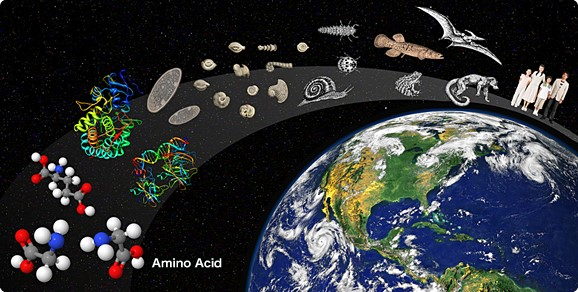
\includegraphics[width=\textwidth]{OriginOfLife.jpg}
        \caption{Vida através de la historia}
        \label{fig:1}
    \end{figure}

La vida en otros mundos, si existe, podría haber evolucionado a través de tipos similares de eras durante la vida útil de su planeta o estrella. En la siguiente lista, el tiempo se indica en miles de millones de años ($\Gy$).

\begin{itemize}
	\item \textbf{Era Hadeica (4.65 - 3.8)$\Gy$}:  Formación de la superficie de la Tierra; impactos asteroidales masivos. Formación de la Luna. Depósito de océanos. Aparición de agua dulce en tierra.
	\item \textbf{Era Arcaica (3.4 - 2.5)$\Gy$:}  Primera evidencia de organismos unicelulares (3.8$\Gy$). Fotosíntesis (3.8$\Gy$); primeros microfósiles (3.6$\Gy$); 
	primeras bacterias productoras de oxígeno (3.6$\Gy$); primeras alfombras fósiles estromatolíticas (3.0$\Gy$).
	\item \textbf{Era Proterozoica (2.5 $\Gy$ - 550 $\My$):}  La atmósfera se vuelve oxigénica (2.1 $\Gy$); formación activa de montañas;
	los protistas aparecen como la primera vida unicelular compleja (1.8$\Gy$); eucariotas multicelulares (1.0 $\Gy$); Tierra de bola de nieve (850 $\My$); formas de vida ediacáricas florecen (600 $\My$).
	\item \textbf{Era Fanerozoica (550 $\My$ - 65 $\My$):}  Gran diversificación de la vida multicelular en océanos, tierra y aire.
	\item \textbf{Era Cenozoica (65 $\My$ hasta hoy):} Fin de la megafauna de dinosaurios (65 $\My$); surgimiento de las formas de vida mamíferas; evolución humana (5 $\My$); aparecen los humanos modernos (50 000 años)
\end{itemize}

Dadas las duraciones de las diversas eras mencionadas anteriormente, y asumiendo que seleccionó un planeta similar a la Tierra en edad, masa, tamaño y temperatura promedio, ¿qué estimaría para los siguientes porcentajes expresados como porcentajes relativos a la edad del planeta?

\vspace{5mm}
\begin{enumerate}
	\item El porcentaje de tiempo en que el planeta tiene vida de cualquier tipo.
	\item El porcentaje de tiempo en que solo existe vida bacteriana (unicelular).
	\item El porcentaje de tiempo en que las formas de vida son más complejas que las bacterias.
	\item El porcentaje de tiempo en que existieron formas de vida similares a los mamíferos.
	\item El porcentaje de tiempo en que las formas de vida son tan inteligentes como los humanos modernos.
\end{enumerate}

\end{problema}
[2]  \cite{NASA_AstrobiologyMath}

\begin{problema}

\textbf{Las formas de vida terrestres más pequeñas}: Las cosas pequeñas son más fáciles de fabricar que las grandes, y también son más numerosas; 
por lo tanto, si estamos tratando de entender cómo surge la vida, resulta útil encontrar el ejemplo más pequeño de un \textit{ser vivo}. 
En esa búsqueda, los científicos han encontrado bacterias, virus y priones, entre otros objetos biológicos pequeños. 
Esta lista incluye objetos que poseen algunos, pero no todos, de los atributos más básicos de la vida: reproducción, consumo de energía y respiración.

    \begin{figure}[H]
        \centering
        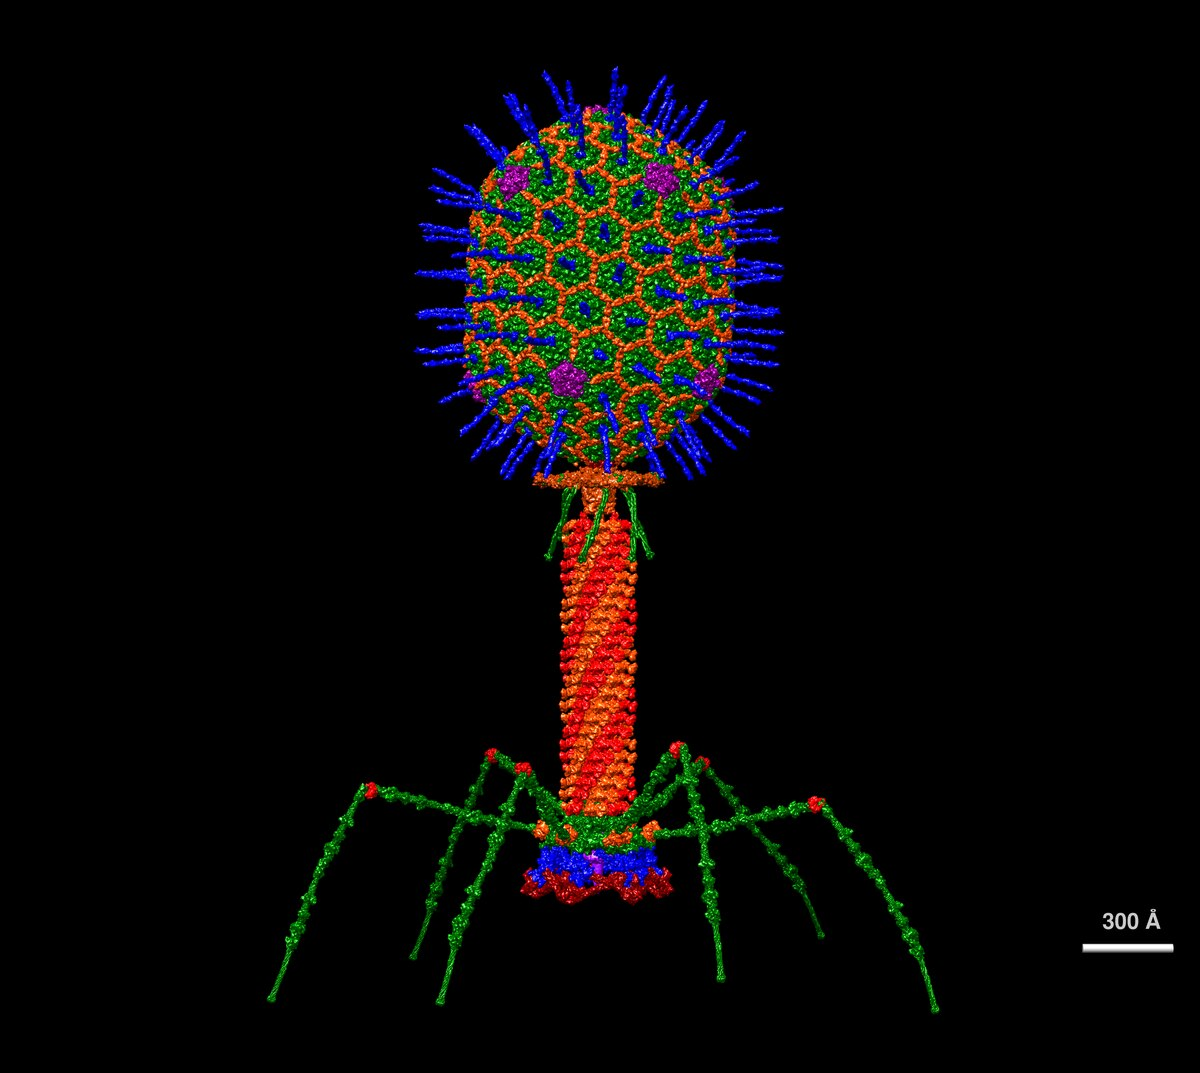
\includegraphics[width=0.6\textwidth]{T4.jpg}
        \caption{Bacteriófago T4, un virus que infecta bacterias. Su estructura compleja —con cabeza icosaédrica, cola contractil y fibras basales— le permite adherirse a la superficie bacteriana e inyectar su material genético.}
        \label{fig:2}
    \end{figure}

La tabla siguiente indica los tamaños en nanómetros ($\nm$) de los objetos vivos y no vivos conocidos. También proporciona el número de genes y el número de nucleótidos en la molécula de ADN (o ARN).

\begin{table}[H]
\centering
\small % Reduce ligeramente el tamaño de fuente
\setlength{\tabcolsep}{4pt} % Reduce espacio entre columnas
\begin{tabularx}{\textwidth}{|L|c|c|c|c|c|}
\hline
\textbf{Name} & \textbf{Tamaño (nm)} & \textbf{Estado} & \textbf{Estructura} & \textbf{Núcleótidos (miles)} & \textbf{Genes} \\
\hline
Porcine Circovirus      & 17   & No vivo    & RNA  & 1.8   & 2    \\
\hline
Hepatitis-B             & 42   & No vivo    & RNA  & 3.0   & 4    \\
\hline
Rous sarcoma Virus      & 80   & No vivo    & RNA  & 3.5   & 3    \\
\hline
Lambda bacteriophage    & 100  & No vivo    & DNA  & 48    & 30   \\
\hline
T4 bacteriophage        & 150  & No vivo    & DNA  & 169   & 160  \\
\hline
Mycoplasma Gen.         & 250  & Vivo       & DNA  & 582   & 521  \\
\hline
Nanoarchaeum Equit.     & 400  & Vivo       & DNA  & 491   & 590  \\
\hline
Escherichia Coli        & 2000 & Vivo       & DNA  & 4000  & 3000 \\
\hline
\end{tabularx}
\caption{Comparación de características genéticas y físicas de sistemas biológicos.}
\label{tab:1}
\end{table}

\vspace{5mm}
\begin{enumerate}
	\item Cuanto más pequeño es un virus o sistema vivo, menos información puede almacenar. 
	Suponga que cada uno de los sistemas en la tabla anterior se puede aproximar como una esfera con el diámetro indicado. 
	Cree un gráfico que muestre el volumen, $V$, del sistema en nanómetros cúbicos $\nm^3$ frente al número, $N$, de nucleótidos (en miles). 
	Como los números serán muy grandes, los valores reales que se grafiquen deben ser los logaritmos en base 10 de $N$ y $V$
	\item Se descubre una forma de vida que tiene aproximadamente 1 000 nucleótidos. ¿Cuál podría ser una clasificación plausible para esta forma de vida: viva o no viva?
	\item Se descubre una forma de vida que tiene un volumen de un billón de nanómetros cúbicos. ¿Cuántos nucleótidos podría tener este organismo?
	\item Suponga que un bacteriófago $T4$ invadió una bacteria \textit{Escherichia Coli} y comenzó a reproducirse hasta que la pared bacteriana se rompió. 
	¿Cuál sería aproximadamente el número máximo de bacteriófagos $T4$ que podrían producirse en el volumen de la bacteria?
\end{enumerate}

\end{problema}
[4]  \cite{NASA_AstrobiologyMath}

\begin{problema}
\textbf{La evolución de los nucleótidos y los genes:} La molécula de ADN de los animales avanzados consiste en millones de nucleótidos que \textit{codifican} aminoácidos específicos 
en el ensamblaje de grandes moléculas llamadas proteínas, que son esenciales para los sistemas vivos. 
Cada proteína está codificada por una cadena de miles de nucleótidos que forman una unidad llamada gen. 
Decenas de miles de genes se encuentran en las moléculas de ADN, que pueden activarse individualmente o en grupos para realizar funciones esenciales para las células vivas.

    \begin{figure}[H]
        \centering
        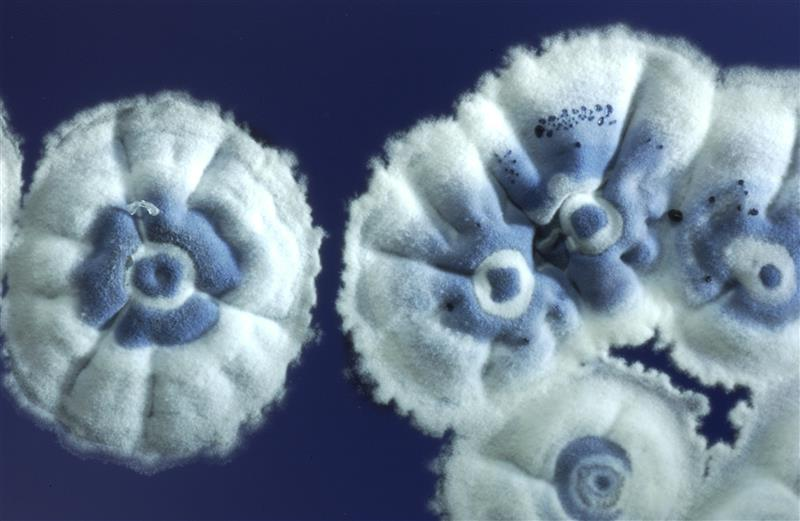
\includegraphics[width=0.7\textwidth]{Coelicolor.jpeg}
        \caption{Streptomyces coelicolor, una bacteria del suelo conocida por su estructura filamentosa y su capacidad para producir antibióticos. Su crecimiento en placas forma colonias con patrones florales característicos.}
        \label{fig:3}
    \end{figure}


Desde 1990, miles de organismos han tenido sus \textit{genes secuenciados}. La tabla siguiente muestra los detalles de algunos organismos comunes.

\begin{table}[H]
\centering
\begin{tabular}{|l|c|c|c|c|}
\hline
\textbf{Especie} & \textbf{Tipo} & \textbf{Edad ($\My$)} & \textbf{Nucleótidos} & \textbf{Genes} \\
\hline
Humano            & Mamífero     & 1       & 2.9 mil millones & 23,000 \\
\hline
Ratón             & Mamífero     & 75      & 3.4 mil millones & 23,000 \\
\hline
Arroz             & Planta       & 100     & 390 millones     & 28,300 \\
\hline
E. Coli           & Bacteria     & 150     & 4.6 millones     & 4,400  \\
\hline
Pez cebra         & Peces        & 300     & 1.2 mil millones & 15,760 \\
\hline
Naegleria Gruberi & Ameba        & 1,000   & 41 millones      & 15,727 \\
\hline
Streptomyces Coelicolor & Bacteria & 450   & 6.7 millones     & 7,842  \\
\hline
Mosca de la fruta & Insecto      & 250     & 122 millones     & 17,000 \\
\hline
Erizo de mar      & Molusco      & 300     & 814 millones     & 23,300 \\
\hline
Helicobacter Pylori & Bacteria   & 150     & 1.7 millones     & 1,589  \\
\hline
\end{tabular}
\caption{Evolución de nucleótidos y genes en organismos comunes.}
\label{tab:2}
\end{table}


\begin{enumerate}
	\item Grafique el número de genes (en unidades de miles) frente al tiempo (en unidades de 100 millones de años). 
	¿Cuál es aproximadamente la tasa de cambio del número de genes por cada cien millones de años hasta la actualidad?
	\item Grafique el número de nucleótidos (en millones) frente al tiempo (en unidades de 100 millones de años). 
	¿Cuál es aproximadamente la tasa de cambio en el número de nucleótidos por cada cien millones de años hasta la actualidad?
	\item Suponga que se descubrió un planeta que, en promedio, tuvo el mismo tipo de evolución biológica que la Tierra durante sus primeros 4.6 mil millones de años, 
	pero hoy en día tiene una edad de 7 mil millones de años. ¿Qué estimaría como el número de nucleótidos y genes para sus organismos más avanzados?
\end{enumerate}
\end{problema}
[10] \cite{NASA_AstrobiologyMath}

\bibliographystyle{plainurl}
\bibliography{bibliografia} % Nombre del .bib

\end{document}
